\section{Accesibiltà}

Il sito mantiene la completa separazione tra struttura, presentazione e comportamento. La struttura è stata sviluppata tramite documenti xHTML, i quali richiamano i fogli di stile esterni CSS puri che implementano la presentazione, ed infine, per quanto riguarda il comportamento, sia script esterni realizzati con JavaScript che pagine dinamiche in PHP.
Tutto il codice redatto è stato scritto secondo le raccomandazioni W3C WCAG 2.0 (Level AAA).
Si sono evitati tag e attributi deprecati. \\

\subsection{Screen reader}
Sono stati effettuati vari test tramite screen reader, cercando il più possibile di simulare l’esperienza di un non vedente sul nostro sito. Così facendo sono state individuate le criticità e sono state quindi sviluppate tecniche per risolverle. \\


La criticità più fastidiosa era data dalla mancanza di \textit{skipLink} efficaci;
sono quindi stati introdotti 3 diversi \textit{skipLink}:
\begin{itemize}
\item Il primo è posto all’inizio della pagina e fa saltare il logo e la navbar, andando al contenuto principale della pagina stessa;
\item Il secondo è presente solo nella pagina contatti e permette di saltare la mappa di Google Maps;
\item Il terzo è posto poco prima del footer e riporta l’utente alla barra di navigazione. Si è pensato infatti che l’utente, dopo aver visitato l’intera pagina, voglia poterne visitare un’altra e viene quindi ridirezionato al menù di navigazione stesso. \\ 
\end{itemize}



Lo \textit{slideshow} è stato programmato in modo da non creare fastidi ai non vedenti. A tal proposito è stato illuminante il seminario svolto in classe.
Il nostro \textit{slideshow} infatti non reagisce con lo screen reader, poiché non cambia in automatico le immagini. Viene inoltre data la possibilità di saltarlo direttamente tramite \textit{skipLink.}\\

Le parole in lingue diverse da quella italiana sono state racchiuse all'interno di tag con l'attributo \textit{lang}, per permettere una corretta lettura da parte dello screen reader.\\


Abbiamo infine provato a navigare i form senza l’uso del mouse e siamo rimasti soddisfatti dal risultato dopo aver corretto vari errori nell’HTML.
I \textit{radio button} che normalmente sono colorati di verde se un’ora è disponibile, o di rosso se invece non lo è (totalmente inutile in caso di disabilità visiva), sono stati modificati aggiungendo l'attributo \textit{disabled="disabled"} facendo in modo che al passaggio sul form il pulsante dichiari il suo stato di disabilitato o meno.
Inoltre, solo con JavaScript attivato, per la segnalazione degli errori, abbiamo deciso di far apparire il messaggio d'errore immediatamente sotto al campo dei form dove è presente l'errore. Questo è stato fatto per poter far leggere subito allo screen reader che errore è stato commesso. 

\pagebreak

\subsection{Colori}

I colori, a tema medico, sono stati scelti in modo da seguire le regole del contrasto e raggiungono un livello di accettabilità tripla A. (In particolare, ratio 7.14:1 tra \#2E5894 e \#FFFFFF, e di 14.39:1 tra \#192168 e \#FFFFFF).
Questi inoltre restano ben distinti anche usando una scala di grigi o con alterazione/mancanza di colori.\\

\begin{center}
\fbox{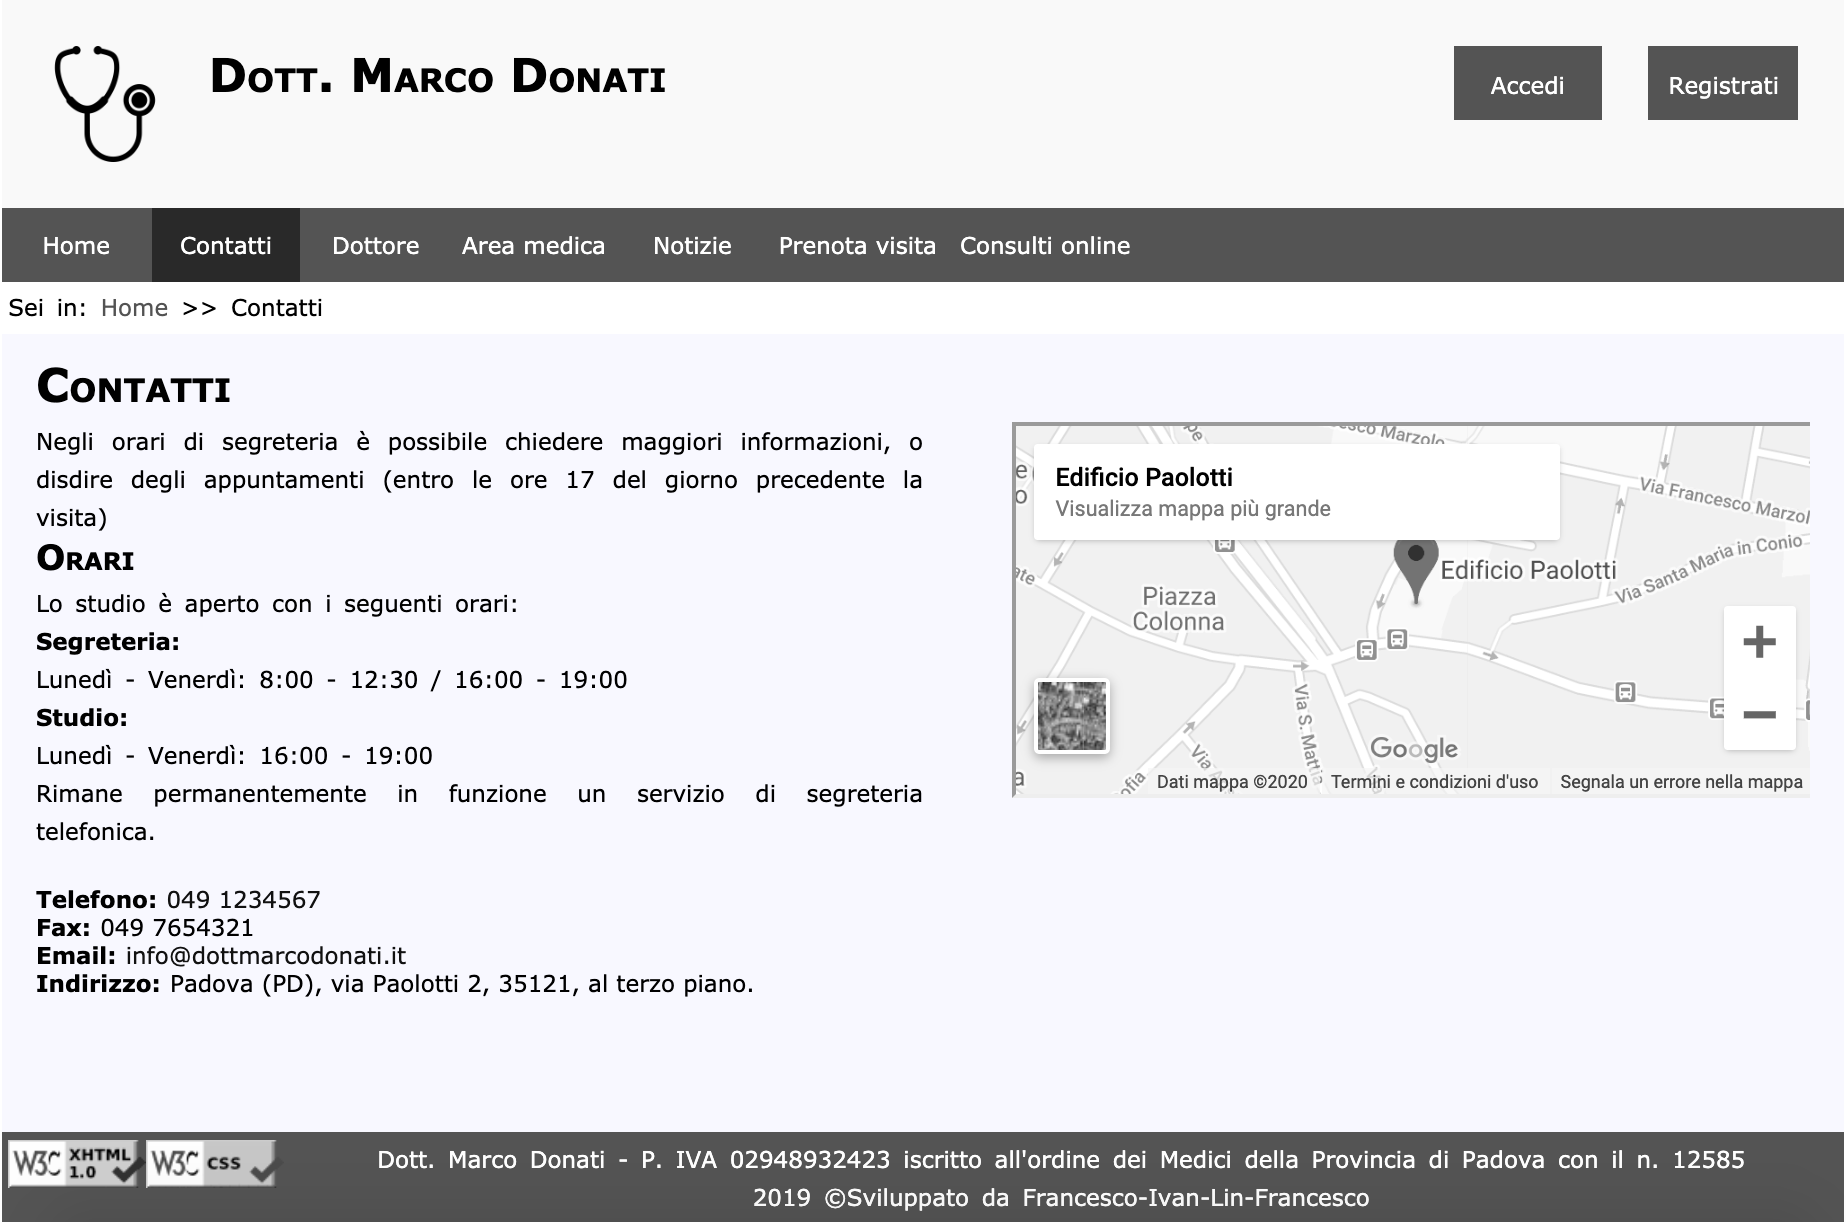
\includegraphics[width=12cm]{../img/bw}}
\end{center}
\captionof{figure}{\textit{Color greatly reduced}}

\bigskip

\begin{center}
\fbox{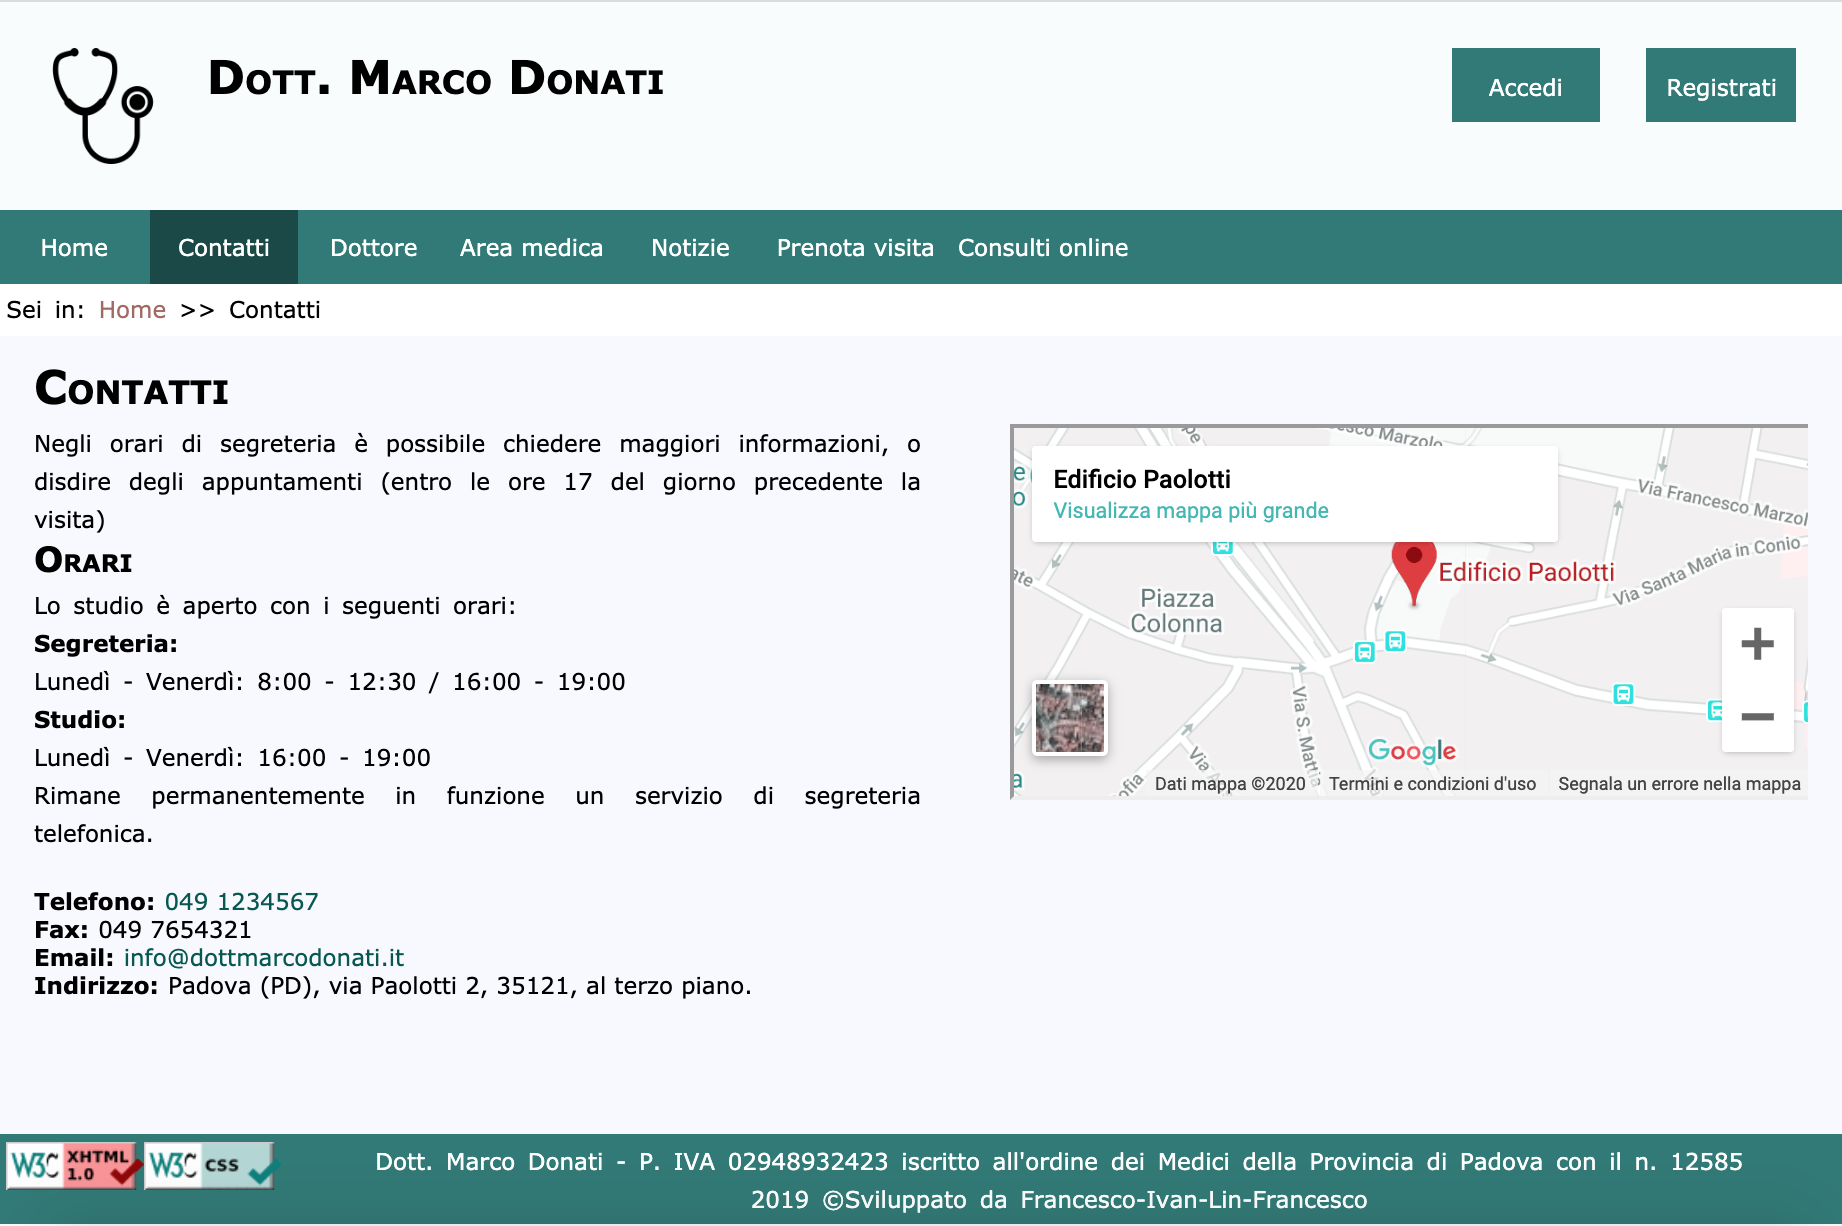
\includegraphics[width=12cm]{../img/green}}
\end{center}
\captionof{figure}{\textit{Blue greatly reduced}}
\subsection{Test}

Tutti i test riguardanti l’accessibilità sono stati svolti (e passati) con:
\begin{itemize}
\item \textit{Total Validator;}
\item \textit{Silktide Screen Reader Simulator;}
\item \textit{Color Contrast Analyzer};
\item \textit{Wawe.}
\end{itemize}

I feedback dati da questi test ci hanno quindi permesso di redarre le sezioni riguardanti l'accessibilità.

